\documentclass[11pt, oneside]{article}   	% use "amsart" instead of "article" for AMSLaTeX format
\usepackage[left=1.5in, right=1.5in, top=1in, bottom=1.5in]{geometry}                		% See geometry.pdf to learn the layout options. There are lots.
\geometry{letterpaper}                   		% ... or a4paper or a5paper or ... 
%\geometry{landscape}                		% Activate for rotated page geometry
%\usepackage[parfill]{parskip}    		% Activate to begin paragraphs with an empty line rather than an indent
\usepackage{graphicx}				% Use pdf, png, jpg, or eps§ with pdflatex; use eps in DVI mode
								% TeX will automatically convert eps --> pdf in pdflatex		
\usepackage{amssymb}
\usepackage{caption}
\usepackage{hyperref}
\usepackage{amsmath}
\usepackage{setspace}  % For custom line spacing

%SetFonts

\setstretch{1.26}  % Change the value here to control the line spacing

%SetFonts


\title{Enhancing Fraud Detection with Quantum Machine Learning: A Comparative Study of Quantum and Classical Approaches}	
\author{William Jasmine \\william.jasmine06@spsmail.cuny.edu}
\date{2024-10-25}							% Activate to display a given date or no date

\begin{document}
\maketitle

\begin{abstract}
Include abstract once results are finalized...
\end{abstract}

\section{Introduction}

\hspace{10mm}Recent years have seen groundbreaking research in both machine learning and quantum computing, positioning these fields at the forefront of some of the most anticipated scientific breakthroughs. Quantum computers promise to solve problems once deemed unsolvable by classical computing, while advancements in generative AI are poised to spark the next major technological revolution, with tech companies racing to develop and deploy their own AI-driven solutions. While much of the excitement around each field has largely remained within their respective domains, researchers have been able to combine components of each to create what are known as quantum machine learning (QML) models. QML combines the processing power of quantum computing with existing machine learning models in an effort to theoretically optimize both their performance and speed.\\

\noindent\hspace{10mm}The work presented here showcases how QML can be used to predict credit card fraud as an example of its potential fraud detection capabilities. Fraud detection has become an increasingly important area of research in recent years, given that the methodologies and techniques used by fraudsters are continuously evolving and pose novel, complex challenges to traditional detection systems. As such, QML can be a possible solution to fight back against these increasingly sophisticated fraudulent attacks. \\

\noindent\hspace{10mm}Using IBM’s QasmSimulator, various aspects of simulated quantum circuits were examined in order to model how different system parameters affected the results of the QML algorithms that they implemented. Once the ideal parameters were determined, QML algorithms were used to predict the presence of fraud in credit card transactions. These results were then compared to those generated using classical machine learning (ML) algorithms. This project focuses on two ML algorithms in particular - Support Vector Machines (SVM) and Random Forests (RF) - along with their QML counterparts - Quantum Support Vector Machines (QSVM) and Quantum Random Forests (QRF). 

\section{Literature Review}

\noindent\hspace{10mm}While being a relatively new field, QML has still seen a number of groundbreaking developments over the years that demonstrate how quantum mechanics can be adapted to tackle complex data processing tasks. Using quantum computers to solve classification problems was explored as early as the late 1990's, in which \href{https://arxiv.org/abs/quant-ph/9706062}{Farhi et al. (1998)} theorized how quantum computers could be used to build decision tress. Later, \href{https://arxiv.org/abs/1907.06840}{Khadiev et al. (2019)} showed how using Grover's algorithm (also known as the quantum search algorithm) could be exploited to improve the efficacy of quantum decision trees, laying the groundwork for their team to be able to eventually demonstrate how to build QRFs in practice \href{https://arxiv.org/abs/2112.13346}{(Khadiev et al. (2021)}). Most recently, QRFs that utilize ``quantum kernels" have been shown to further enhance their ability to process and analyze data, first evidenced by \href{https://arxiv.org/abs/2210.02355}{Srikumar et al. (2022)}. \\

\noindent\hspace{10mm}Research on how to apply quantum enhancements to machine learning has been extended to numerous additional algorithms, including support vector machines (SVMs). In the early 2000s \href{https://members.cbio.mines-paristech.fr/~jvert/svn/bibli/local/Anguita2003Quantum.pdf}{Anguita et al. (2003)} first laid out the theoretical foundation for how quantum computing could be use to train SVM models. \href{https://arxiv.org/abs/1307.0471}{Rebentrost et al. (2014)} and \href{https://arxiv.org/abs/1612.03713}{Chatterjee et al. (2017)} expanded on this early work to show how QSVMs could be produced in practice by creating quantum versions of the kernel needed by SVM models to transform data into a higher dimensional space. 

\noindent\hspace{10mm} While many other theory-based papers were identified over the course of this literature review, the following comprehensive studies provide brilliant summaries of the numerous techniques and developments seen over the course of QML's relatively brief history: 

\begin{itemize}

\item \href{https://arxiv.org/abs/1611.09347}{Biamonte et al. (2017)} provides a robust review of the theoretical framework behind QSVM and the potential benefits that can be achieved when compared to using traditional SVMs. 
\item \href{https://pubmed.ncbi.nlm.nih.gov/36832654/}{Zeguendry et al. (2023)} provides a concise overview of the quantum mechanics involved in building QML algorithms and provides numerous case studies of how these algorithms can be applied in practice. 


\end{itemize}

\noindent\hspace{10mm}Each of the above papers have numerous citations and were used as key points of reference while completing the work presented here. \\

\noindent\hspace{10mm}There are also numerous instances of instances in which QML algorithms are applied to real world scenarios to test the potential upsides speculated in the aforementioned theoretical research. The list below includes some noteworthy examples: 

\begin{itemize}

\item Shan et al. (2022) used QSVMs as a methodology for breast cancer detection and show that it can match accuracy results comparable to that of classical SVMs.
\item Luo et al. (2024) have shown that QML algorithms have ``promising potential" when being used to predict predict the presence of Alzheimer's disease, though have not yet surpassed their classical counterparts in terms of learning capability.  
\item Cherrat et al. (2023) were able to develop a reinforcement learning model via Quantum Neural Networks (QNNs) and used financial sector data to tackle the problem of hedging. 

\end{itemize}

\noindent\hspace{10mm}Numerous additional case studies of QML are summarized in a study done by \href{https://arxiv.org/abs/2406.13262}{Nguyen et al. (2024)}, which draws on the findings from 32 previously written papers in the field that give a robust summary of the potential upside that can be realized when switching to use QML algorithms. This paper was also used as a consistent point of reference when completing the work presented here. A review of these numerous case studies reveals that QML algorithms either very nearly approach of exceed the performance seen from classical ML algorithms, fostering excitement when considering the prospect of applying these findings specifically to the realm of fraud detection. \\

\noindent\hspace{10mm}That being said, there is already some existing work that shows how quantum machine learning can be used in fraud detection problems. Namely, \href{https://arxiv.org/abs/2308.05237}{Innan et al. 2023} show that QSVMs seem to outperform Quantum Neural Network (QNN) algorithms when solving fraud detection problems, while \href{https://arxiv.org/abs/2208.01203}{Kyriienko et al. (2022)} show that QSVMs have similar performance compared to classical SVMs when trying to identify fraudulent banking transactions. That being said, the purpose of this work is to extend beyond the existing research to specifically quantify how changing the features of a quantum circuit affect the results of both the and QSVM and QRF algorithms in regards to predicting credit card fraud, and compare the results of \textit{both} algorithms against those of their classical counterparts.\\

\noindent\hspace{10mm}It is worth noting that as of July 2024, it has been revealed that \href{https://thequantuminsider.com/2024/07/19/deloitte-italy-explores-quantum-machine-learning-for-digital-payments-fraud-detection/}{Deloitte is exploring using QML (specifically, QNNs) to detect fraudulent online payments}. While they have provided no study of their results, the work presented here could provide quantitative evidence that utilizing QML should be considered as a possible next step in the ongoing fight against fraud. 

\section{Hypothesis}

Given the findings of the literature review, it appears clear that QSVMs should approach or exceed the performance of a classical SVM model in identifying credit card fraud, especially after the best quantum circuit for the scenario has been identified. Given the arguably superior ability of RFs over SVMs to handle high dimensional feature spaces, it is expected that QRFs should be able to build on the gains realized by QSVMs. Once again, this is only after the best tuned quantum circuit has been identified. Identifying these ideal quantum circuits, will be an exercise in balancing complexity: adding to the circuit's ability to handle more complex data structures (by increasing the number of qubits, using more expansive entanglement patterns etc.) will likely increase model performance up a point, but will eventually witness decreased efficiency and suffer from added noise. 

\section{Data}
\subsection{Data Source}

\hspace{10mm}The dataset used in this project is \href{https://www.kaggle.com/datasets/nelgiriyewithana/credit-card-fraud-detection-dataset-2023}{sourced from Kaggle} and contains data of over 550,000 credit card transactions in the EU during 2023. The original source of the data is the result of a \href{https://www.researchgate.net/publication/283349138_Calibrating_Probability_with_Undersampling_for_Unbalanced_Classification}{research collaboration} between Worldline and the Machine Learning Group of ULB (Université Libre de Bruxelles). The data is anonymized to protect the identity of the credit card users and contains 29 predictor variables representing various aspects of each credit card transaction.  Due to the anonymization, it is impossible to know exactly what each of these first 28 features represent (they are all labelled simply as V1 through V28), but it is shared that they represent the commonly captured features of a credit card transaction (i.e. time, location, etc.). These first 28 features have all been transformed to be continuous numerical features. The only titled predictor variable in the dataset is ``Amount", which represents the total amount of the credit card transaction in Euros. The goal when using this dataset will be to predict ``Class”, a binary field indicating whether or not the transaction was fraudulent.

\subsection{Data Cleaning}

\hspace{10mm}Datasets for this project were considered only if they had a reputation for being clean and usable, ensuring the focus remains on model performance rather than being heavily influenced by data cleaning, imputation, or collection methods. As such, this dataset contains 568,630 records in which none of the fields have missing, misprinted, or nan values. The target variable, ``Class", contains either 1 or 0, indicating whether the observation is fraudulent (1) or valid (0). \\


\begin{figure}[h!]
    \centering
    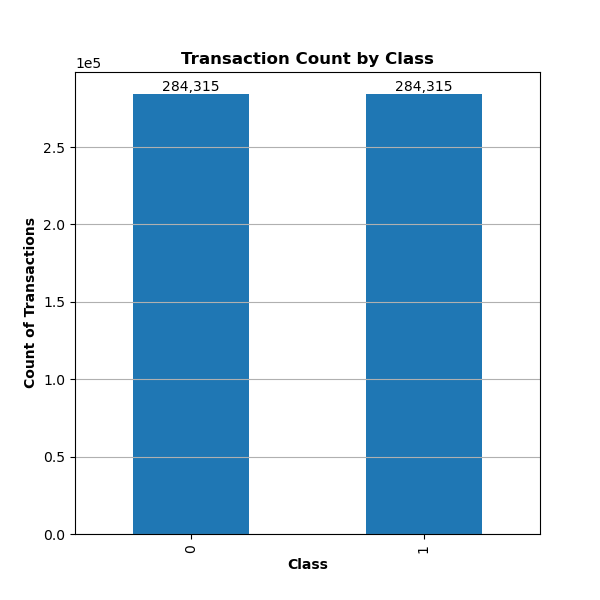
\includegraphics[width=0.6\textwidth]{figures/fig_1.png}
    \captionsetup{font=small} 
    \caption{There are an equal number of fraudulent (1) and valid (0) transactions in the initial dataset.}
    \label{fig1}
\end{figure}


\noindent\hspace{10mm}However, Figure 1 does highlight a different type of issue with the dataset: balanced classes. Though the balanced dataset might make it easier to predict instances of fraud, it is not representative of what occurs in the real world. The European Banking Authority (EBA) estimates that \href{https://www.eba.europa.eu/sites/default/files/2024-08/465e3044-4773-4e9d-8ca8-b1cd031295fc/EBA_ECB\%202024\%20Report\%20on\%20Payment\%20Fraud.pdf}{``fraud accounted for 0.031\% of total card payments in value and 0.015\% of total card payments in volume terms in H1 2023"}. As such, in order to mimic a more realistic scenario, observations representing fraudulent transactions were randomly removed until they represented only 1\% of total transactions. Although the percentage of fraudulent transactions is still inflated compared to the estimate made by the EBA, this update shifts the machine learning objective to actual fraud detection while ensuring that a sufficient number of fraudulent samples are retained. Figure 2 shows the the updated version of transactions by class after the change.\\

\begin{figure}[h!]
    \centering
    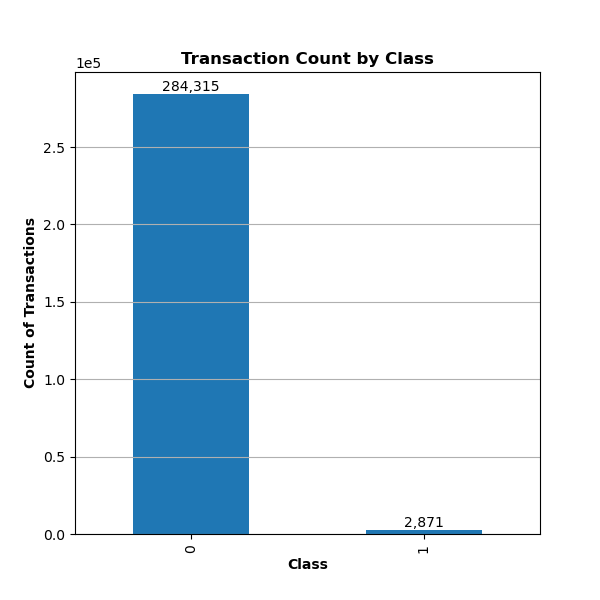
\includegraphics[width=0.6\textwidth]{figures/fig_2.png}
    \captionsetup{font=small} 
    \caption{The updated breakdown by class represents a paints a more realistic picture of credit card fraud, and still maintains a decent number of fraudulent transactions.}
    \label{fig2}
\end{figure}

\noindent\hspace{10mm}Figure 3 shows the distribution of all 28 of the anonymized predictor variables (V1-V28), which all appear to have similar scale. However, the sole remaining titled predictor variable has not been transformed in any way meaning that it has a range much larger than those of the predictors seen in Figure 3. Given that the SVM algorithms implemented in this study are sensitive to scale, a Min-Max scaler was applied to set the range of all features between 0 and 1. Figure 4 shows the distribution of all predictor variables after the scaler has been applied. 

\begin{figure}[h!]
    \centering
    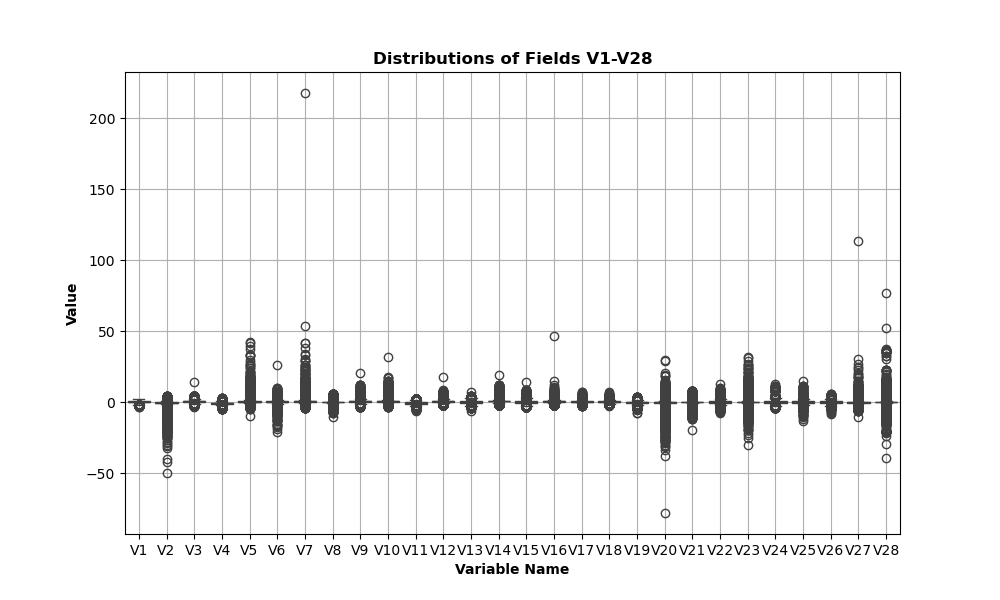
\includegraphics[width=1.0\textwidth]{figures/fig_3.png}
    \captionsetup{font=small} 
    \caption{The transformation applied to the anonymized predictor variables results in 28 fields that all appear to similar scale.}
    \label{fig3}
\end{figure}

\begin{figure}[h!]
    \centering
    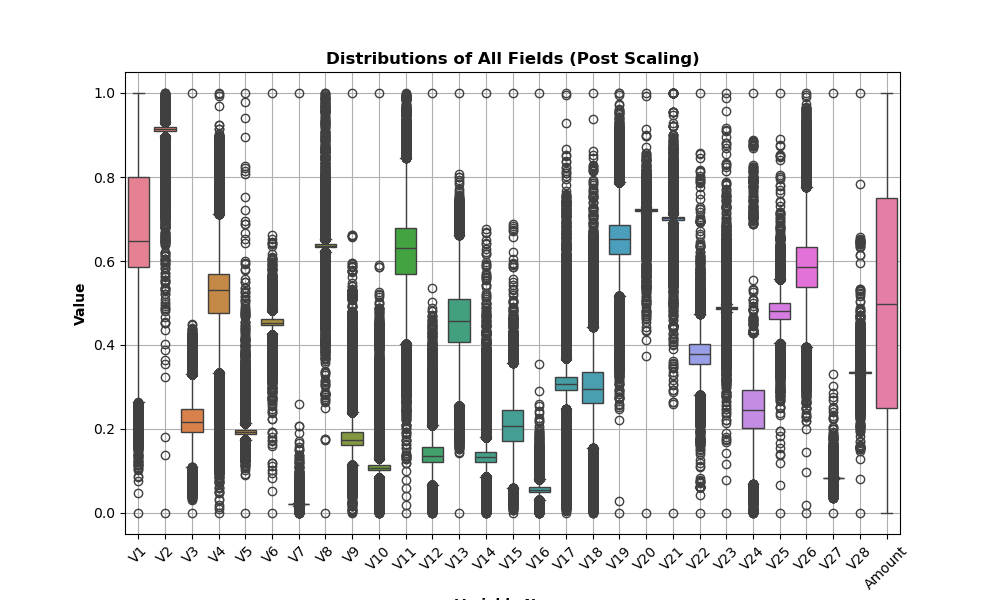
\includegraphics[width=1.0\textwidth]{figures/fig_4.png}
    \captionsetup{font=small} 
    \caption{All 29 predictor variables have a range between 0 and 1 after the min-max scaler has been applied. This change should result in more accurate predictions from ML algorithms that are sensitive to scale.}
    \label{fig4}
\end{figure}	

\subsection{Exploratory Data Analysis}

Before applying any machine learning models to the data, an initial analysis was completed in an effort to determine which of the explanatory variables might be useful in making predictions. To do this, $t$-tests were performed that compared the difference of means for each field when separated by class. Figure 5 shows the results of these $t$-tests, which show that 26 of the 29 explanatory fields exhibited statistically significant differences when comparing the means of each variable by class.  

\begin{figure}[h!]
    \centering
    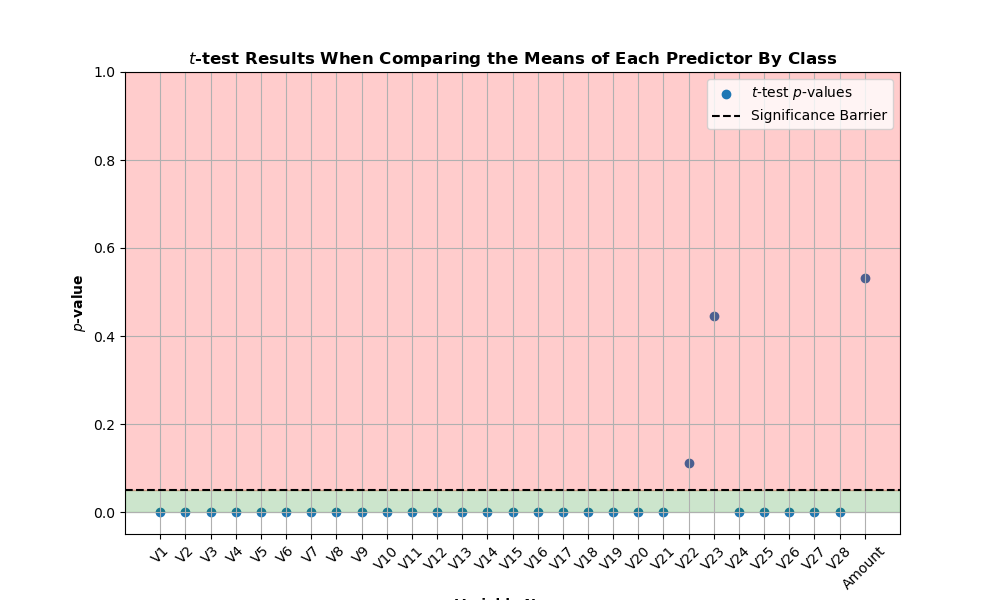
\includegraphics[width=1.0\textwidth]{figures/fig_5.png}
    \captionsetup{font=small} 
    \caption{26 of the 29 explanatory fields exhibited statistically significant differences when comparing the means of each variable by class.}
    \label{fig5}
\end{figure}

Indeed, Figure 6 uses the V1 field as an example to show that a comparison of the distributions by class reveals a stark difference. 

\begin{figure}[h!]
    \centering
    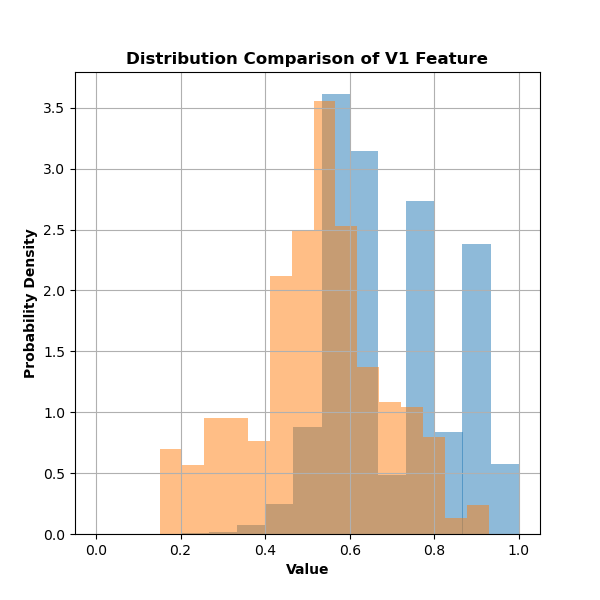
\includegraphics[width=0.6\textwidth]{figures/fig_6.png}
    \captionsetup{font=small} 
    \caption{The V1 field was identified as a having a statistically significant difference when comparing the means of the observations in each class. The reason why is clear in the figure, with the probability density distributions of each class being disparate.}
    \label{fig6}
\end{figure}

This results of this analysis bode well for the quality of this dataset, as it appears to contain features that will be useful in making predictions on the target variable. It provides confidence that identifying the fraudulent transactions via ML algorithms is possible.

\section{Methods}
\subsection{Quantum Computer Simulation}

\hspace{10mm}Quantum computing is still in its infancy in regards to mainstream accessibility and usage, with IBM appearing to be one of the only companies offering the ability to run jobs on utility scale quantum computers. That being said, their most limited plan comes at a cost of \href{https://www.ibm.com/quantum/pricing}{\$96 per minute of runtime}, which is outside the realm of feasibility for this project. Thankfully, the open source python package IBM maintains to handle all requests for their quantum computers (known as \href{https://www.ibm.com/quantum/qiskit#get-started}{Qiskit}) allows the use of quantum simulators for free. IBM’s \href{https://qiskit.github.io/qiskit-aer/stubs/qiskit_aer.QasmSimulator.html}{QasmSimulator} uses classical computing to mimic the output produced by their quantum computers by using mathematics stemming from quantum mechanics to calculate how the qubits evolve over time. \\

\noindent\hspace{10mm}Given the apparent legitimacy of the work done to produce them, these quantum simulators are an accepted gateway used by students and researchers alike to begin their journey into the world of quantum computing and there is \href{https://www6.slac.stanford.edu/news/2023-01-30-researchers-take-step-toward-novel-quantum-simulators}{evidence of them being used for published research in the field}. Thus, this project will rely on IBM’s QasmSimulator to create the quantum systems that implement the QML algorithms being studied.


\subsection{Classical ML Algorithms}

\hspace{10mm}This subsection includes descriptions of the classical ML algorithms used in this project, and how they were implemented. 

\subsubsection{Support Vector Machines (SVM)}

\hspace{10mm}Support Vector Machines (SVM) are a type of supervised learning algorithm used for classification tasks, especially when the data is not linearly separable. The key idea behind SVM is to find the hyperplane that best separates the data into different classes. More specifically, SVM attempts to find the hyperplane that maximizes what's known as the \textit{margin} - the distance between the hyperplane and the nearest data points from each class (these distances are the ``support vectors"). In a simple two-dimensional space, this hyperplane is essentially a line that divides the data points, but in higher-dimensional spaces, it becomes a complex multidimensional boundary.  To enable this, SVM uses a kernel function that transforms the data into a higher-dimensional space where it is more likely to for the classes to be linearly separable. Once the best hyperplane is identified, the SVM classifier can use this boundary to classify new data points.\\

\noindent\hspace{10mm}SVMs are a classic option when solving classification problems, and was one of the first to be adapted to be used on quantum computers according to the literature review. Consequently, they emerged as a clear choice when determining which ML algorithms to evaluate in this project. The SVMs models presented here are all implemented using Python, which, thanks to the \href{https://scikit-learn.org/stable/}{scikit-learn library},  makes model creation, training, and validation all very straightforward.


\subsubsection{Random Forests (RF)}

\hspace{10mm}Random Forests belong to family of ML algorithms known as ensemble learning methods, which mean they combine the output of several simpler models - decision trees in case of the random forest - to improve accuracy. Each decision tree in a Random Forest is trained on a different, random subset of the data, introducing randomness that helps to limit overfitting (a common problem with individual decision trees). By taking a majority vote across all trees, Random Forests create a more stable and generalizable model compared to using just one decision tree. In addition, this ensemble or averaging methodology gives Random Forests a reputation for being models that can reduce variance while maintaining low bias. \\

\noindent\hspace{10mm}Random forests tend to have the advantage over SVMs when it comes to dealing with many features and complex pattern recognition. As such, they were chosen as a candidate to evaluate if their quantum counterparts (QRFs) could provide added benefits in regards to fraud detection, given that there is already some evidence of QSVMs being successful in this area. In addition to SVMs, the python \href{https://scikit-learn.org/stable/}{scikit-learn library} also allows for easy implementation of Random Forests.

\subsection{QML Algorithms}

\hspace{10mm}This subsection includes descriptions of the QML algorithms used in this project, and how they were implemented. In addition, it aims to explain how each is an extension of its analogous classical ML version.

\subsubsection{Quantum Support Vector Machines (QSVM)}

\hspace{10mm}Quantum Support Vector Machines (QSVM) are an extension of the classical SVM algorithm, designed to leverage the unique properties of quantum computing. While classical SVMs aim to find a hyperplane that best separates data points into classes, QSVM goes a step further by using quantum feature maps to project the input data into a high-dimensional quantum Hilbert space. This enables QSVMs to identify more complex decision boundaries that classical SVMs may not be able to determine efficiently. Instead of mapping data with traditional kernel functions, QSVMs use quantum circuits to transform the data into quantum states. These quantum states are then used to calculate the \textit{quantum kernel}, which determines the similarity between data points in the quantum feature space. \\

\noindent\hspace{10mm}Despite the apparent complexity of this model, implementing QSVM is made accessible through IBM’s Qiskit framework, which utilizes methods such as ZZFeatureMap and QuantumKernel to make classifications.


\subsubsection{Quantum Random Forests (QRF)}

\hspace{10mm} A quantum Random Forests (QRF) is an extension of a classical random forest, designed to leverage the principles of quantum computing to enhance decision-making processes. Just like traditional random forests, QRFs are an ensemble learning method that builds upon many simpler models, each trained on random subsets of the data, and aggregates their predictions to improve accuracy and reduce overfitting. However, unlike the decision trees that are used to build classical Random Forests, each ``tree" in a Quantum Random Forest is effectively a quantum circuit that performs classification based on the quantum features of the input data. The inherent properties of quantum mechanics, such as superposition and entanglement, allow QRFs to model complex relationships within the data. \\

\noindent\hspace{10mm} Once again, IBM’s Qiskit framework makes it possible to implement Quantum Random Forests, this time by utilizing the QuantumRandomForestClassifier method.

\subsection{Experimental Setup}

\hspace{10mm}The goal of this project is twofold: 

\begin{enumerate}
    \item To model how changing various parameters of a quantum computing system (quantum circuit) affects the quality of predictions made by QSVM and QRF models.
    \item Use the results of completing the first goal to build optimized quantum circuits to implement QSVM and QRF models, and compare the results of their predictions to those produced by tuned versions of their classical counterparts.
\end{enumerate}

\noindent\hspace{10mm}The first goal is achieved by analyzing how the results of predictions made by QML algorithms vary when changing the various parameters needed to build a quantum circuit. These include parameters include:


\begin{itemize}
    \item \textbf{Qubits:} The main components of any quantum circuit are the qubits it contains to actually perform any calculations. Adding qubits to a quantum circuit allows for increased complexity.
    \item \textbf{Repetitions:} Additional repetitions introduce more quantum gates, increasing the depth of the quantum circuit. Changing this parameter is analogous to adding more layers to a neural network, resulting in a more complex system where additional sequential operations are performed on the qubits
    \item \textbf{Entanglement Pattern:} One of the most fascinating aspects of quantum mechanics is that it teaches us particles (in this case, qubits) can be entangled with one another so that the state of one qubit directly influences the state of another. Different entanglement patterns in a QML algorithm impact the model’s ability to capture complex correlations in the data.
    \item \textbf{Mapping functions:} These functions determine how classical data is encoded into quantum states, influencing how well the quantum circuit captures patterns in the data. A more complex mapping function can enhance the expressiveness of the model by enabling it to represent intricate relationships.
\end{itemize}

Once the relationship between each of these parameters and model performance is defined, ideal quantum circuits will be built to implement both the QSVM and QRF models. These models will then be used to predict the fraudulent transactions in the dataset, using precision and recall as metrics to evaluate their performance. To see how these results compare against classical machine learning, tuned SVM and RF models will be produced and make predictions on the same data. This will result in completion of the project's second and final goal. 



\end{document}